\documentclass[12pt]{article}
\usepackage{setspace, graphicx, fullpage, amssymb, amsmath, epsfig, natbib, array, multirow, hyperref}
\usepackage{amsfonts, bm} 
\usepackage{dcolumn}
\usepackage{subfigure, float} 
\usepackage[margin=.75in]{geometry} 
\usepackage{verbatim}
\usepackage{url}
\usepackage{enumerate}
\newcolumntype{d}[1]{D{.}{.}{#1}} 

\begin{document}
	
	\begin{center}
		Update: 30 November 2016
	\end{center}

The first goal for the last two weeks was to determine if we could improve upon the previous algorithm specifications by replacing the random reassignment of votes by instead removing what we have come to term as ``flip flop votes'' from the part of our algorithm which calculates $p$-values. While we were able to create parameters for our algorithm which accomplished this, their overall performance for sessions beyond the 100th was worse than all specifications we have tried, including the original simulated annealing. The only advantage it has over the original simulated annealing is that since it lacks randomness in its methods it will not produce different results based on setting a seed, something that we accomplished while also reducing gray votes by randomly reassigning the ``flip flops.'' Below I include a summary graph and table fo the new method while also including the summary stats from the last update for the sake of comparison. The bulk of these are included at the end of the update.

The new specification also does not closely match what we were doing before in terms of classifying votes:

	\begin{table}[!ht]
		\centering
		\caption{Flip Flop Votes Excluded from Ideal Points Vs. Old Coding}
		\begin{tabular}{l c c c}
			\hline
            \hline
            Classification &  New Grays & New Noncalls & New Party Calls \\
            Old Grays      &  530   &  790    &    264 \\
            Old Noncalls  &   500  &  6503    &    525 \\
            Old Party Calls & 398   & 1548    &   4819 \\
            \hline
            $ \chi^{2} = 8103.1 $ & df = 4 & $p$-value = $< 2.2e-16$ & \\
            
   		\end{tabular}
   	\end{table}

I further include the results of tests to determine if the hybrid model is plagued by the problems of different seeds leading to different results as was present in the original simulated annealing only model. Unfortunately, the test-retest of this proved unreliable across different seeds set for these.

	\begin{table}[!ht]
		\centering
		\caption{Hybrid Specifications with Different Seeds Set}
		\begin{tabular}{l c c c}
			\hline
			\hline
			Classification &  Seed 2 Grays & Seed 2 Noncalls & Seed 2 Party Calls \\
			Seed 1 Grays      &  587 &     98    &     47 \\
			Seed 1 Noncalls  &   28  &  7772     &    27 \\
			Seed 1 Party Calls & 57  &   106      & 7162 \\
			\hline
			$ \chi^{2} = 26032 $ & df = 4 & $p$-value = $< 2.2e-16$ & \\
			
		\end{tabular}
	\end{table}

It also differs substantially from a simulated annealing model with the same seed set as shown below.

	\begin{table}[!ht]
		\centering
		\caption{Seed 1: Simulated Annealing vs. Hybrid Specification}
		\begin{tabular}{l c c c}
			\hline
			\hline
			Classification &  Sim. Annealing Grays & Sim. Annealing Noncalls & Sim. Annealing Party Calls \\
			Hybrid Grays      &  579 &    124    &     29 \\
			Hybrid Noncalls  &   187 &   7399    &    241 \\
			Hybrid Party Calls & 362 &    117     &  6846 \\
			\hline
			$ \chi^{2} = 19770$ & df = 4 & $p$-value = $< 2.2e-16$ & \\
			
		\end{tabular}
	\end{table}

	\begin{table}[!ht]
		\centering
		\caption{Seed 2: Simulated Annealing vs. Hybrid Specification}
		\begin{tabular}{l c c c}
			\hline
			\hline
			Classification &  Sim. Annealing Grays & Sim. Annealing Noncalls & Sim. Annealing Party Calls \\
			Hybrid Grays      &  594 &     59    &     19 \\
			Hybrid Noncalls  &   276 &   7671    &     29 \\
			Hybrid Party Calls & 341 &      8    &   6887 \\
			\hline
			$ \chi^{2} = 19770$ & df = 4 & $p$-value = $< 2.2e-16$ & \\
			
		\end{tabular}
	\end{table}

$ $


\begin{figure}[h]
	\caption{Chart of gray vote percent per session in the specification for flip flops removed from ideal points but not randomly reassigned.}
	\centering
	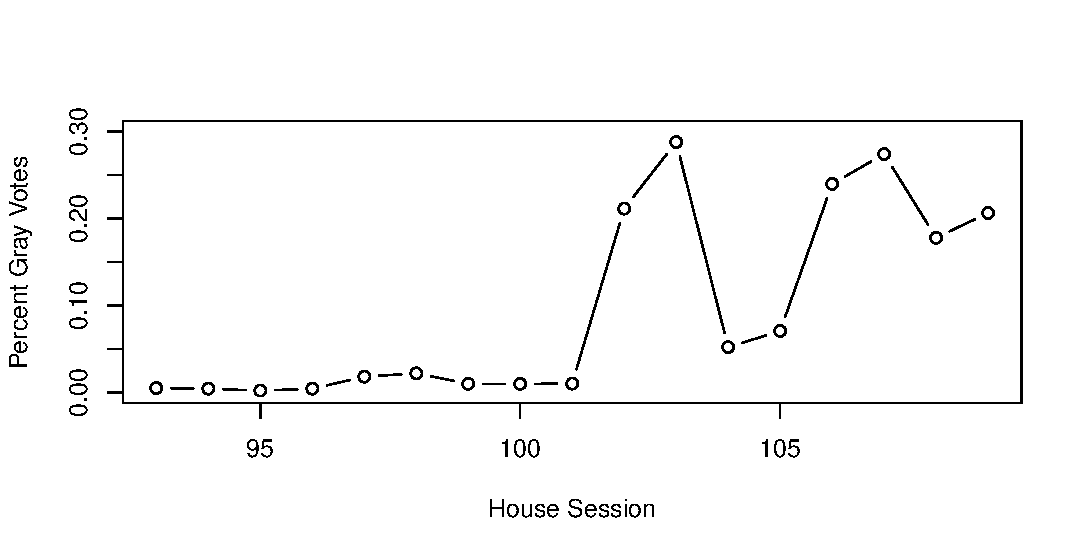
\includegraphics[height=10cm]{C:/Users/Ethan/Documents/GitHub/partycalls/plots/gray_vote_percents_drop_flip_flops_from_ideal.pdf}
	
\end{figure}



\begin{figure}[h]
	
	\caption{Previous Model Gray Vote Percents}
	\centering
	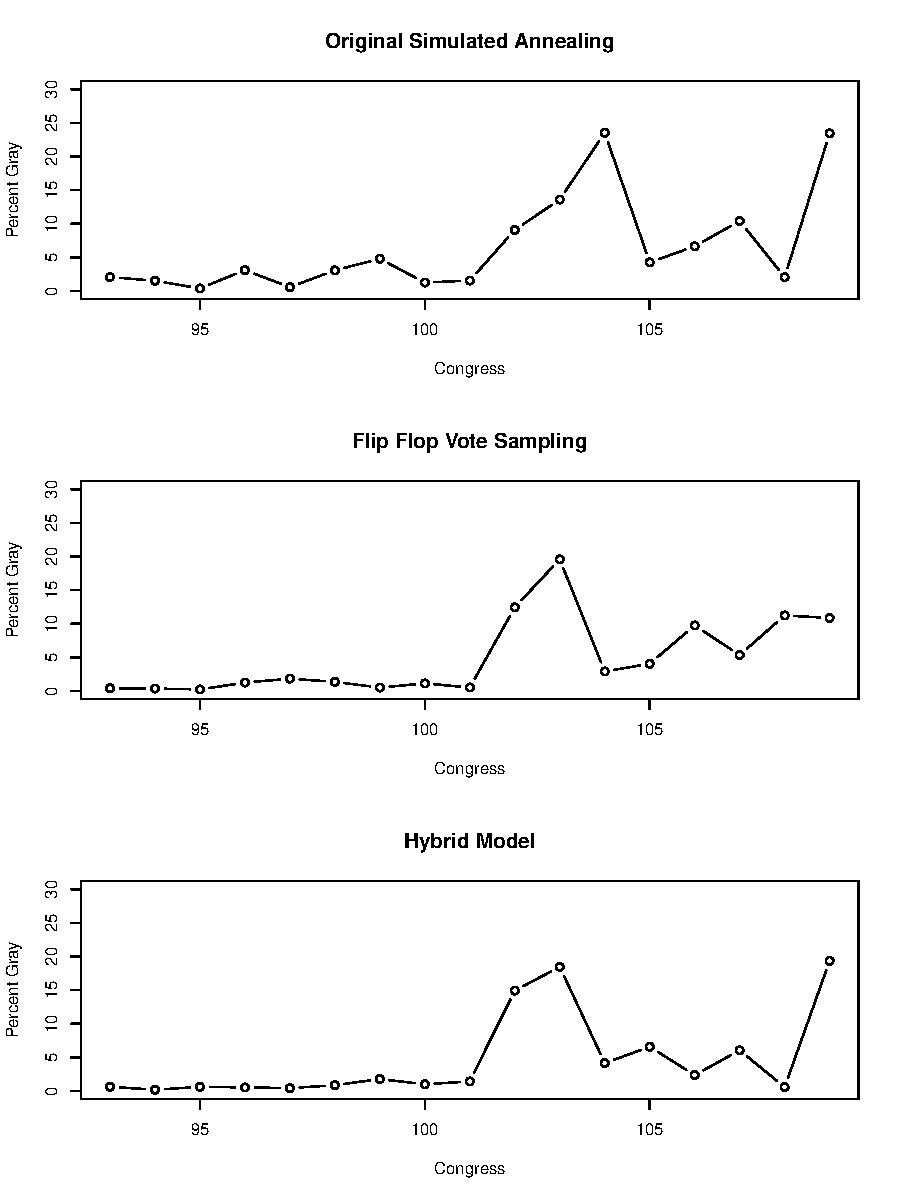
\includegraphics[]{C:/Users/Ethan/Documents/GitHub/partycalls/plots/gray_plot_nov16_1.pdf}
	
\end{figure}

\begin{figure}[h]

\caption{Replication of Figure 2 with Flip Flops Removed from Ideals}
\centering
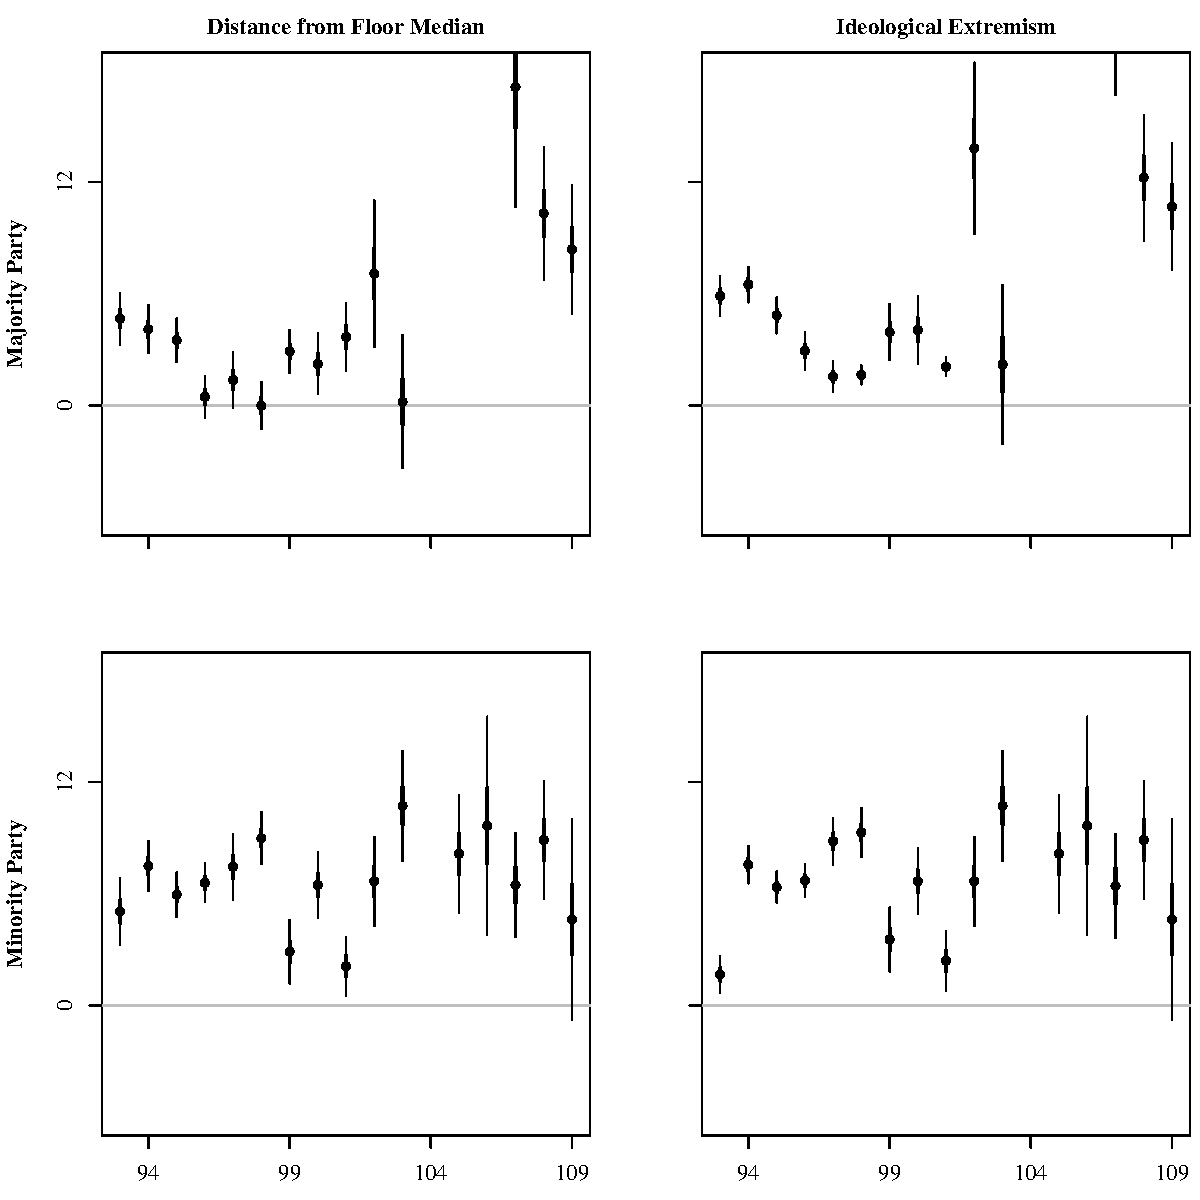
\includegraphics[width = \textwidth]{C:/Users/Ethan/Documents/GitHub/partycalls/plots/replicate-who-heeds-figure2_drop_flip_flops_from_ideal.pdf}

\end{figure}

	\begin{table}[!htbp]
		\centering
		\caption{Flip Flop Votes Excluded from Ideal Points}
		\begin{tabular}{l c}
			\hline
			congress & \% Gray \\ 
			\hline
			93 & 0.5 \\ 
			94 & 0.4 \\ 
			95 & 0.2 \\ 
			96 & 0.4 \\ 
			97 & 1.8 \\ 
			98 & 2.2 \\ 
			99 & 1.0 \\ 
			100 & 1.0 \\ 
			101 & 1.0 \\ 
			102 & 21.1 \\ 
			103 & 28.8 \\ 
			104 & 5.2 \\ 
			105 & 7.1 \\ 
			106 & 24.0 \\ 
			107 & 27.4 \\ 
			108 & 17.8 \\ 
			109 & 20.7 \\ 
			\hline
			Mean: & 9.5 \\
			Median & 2.2 \\
			SD & 10.9 \\
			\hline
		\end{tabular}
	\end{table}
	
	\begin{table}[!htbp]
		\centering
		\caption{Original Simulated Annealing}
		\begin{tabular}{l c}
			\hline
			congress & \% Gray \\ 
			\hline
			93 & 2.1 \\ 
			94 & 1.5 \\ 
			95 & 0.4 \\ 
			96 & 3.1 \\ 
			97 & 0.6 \\ 
			98 & 3.1 \\ 
			99 & 4.8 \\ 
			100 & 1.3 \\ 
			101 & 1.5 \\ 
			102 & 9.1 \\ 
			103 & 13.6 \\ 
			104 & 23.5 \\ 
			105 & 4.3 \\ 
			106 & 6.6 \\ 
			107 & 10.4 \\ 
			108 & 2.0 \\ 
			109 & 23.4 \\ 
			\hline
			Mean: & 6.5 \\
			Median & 3.1 \\
			SD & 7.4 \\
			\hline
		\end{tabular}
	\end{table}
	


	\begin{table}[!htbp]
		\begin{center}
			\caption{Flip Flop Vote Sampling}
			\begin{tabular}[!hb]{lc}
				\hline
				Congress &  \% Gray  \\
				\hline
				
				93 & 0.4 \\ 
				94 & 0.4 \\ 
				95 & 0.2 \\ 
				96 & 1.2 \\ 
				97 & 1.8 \\ 
				98 & 1.4 \\ 
				99 & 0.5 \\ 
				100 & 1.1 \\ 
				101 & 0.5 \\ 
				102 & 12.4 \\ 
				103 & 19.6 \\ 
				104 & 2.9 \\ 
				105 & 4.0 \\ 
				106 & 9.7 \\ 
				107 & 5.3 \\ 
				108 & 11.2 \\ 
				109 & 10.9 \\ 
				\hline
				Mean & 4.9 \\
				Median & 1.8 \\
				SD & 5.7 \\
				\hline
			\end{tabular}
		\end{center}
	\end{table}
	


	\begin{table}[!htbp]
		\begin{center}
			\caption{Hybrid Model}
			\begin{tabular}[!hb]{lc}
				\hline
				Congress &  \% Gray  \\
				\hline
				93 & 0.6 \\ 
				94 & 0.2 \\ 
				95 & 0.6 \\ 
				96 & 0.5 \\ 
			    97 & 0.4 \\ 
				98 & 0.9 \\ 
				99 & 1.8 \\ 
				100 & 1.0 \\ 
				101 & 1.4 \\ 
				102 & 14.9 \\ 
				103 & 18.5 \\ 
				104 & 4.1 \\ 
				105 & 6.6 \\ 
				106 & 2.4 \\ 
				107 & 6.1 \\ 
				108 & 0.6 \\ 
				109 & 19.4 \\ 
				\hline
				Mean & 4.7 \\
				Median & 1.4 \\
				SD & 6.5 \\
				\hline
			\end{tabular}
		\end{center}
	\end{table}
	
	
	

	
	
	
	
	
	
\end{document}